\documentclass{article}

\usepackage{graphicx}
\usepackage{tikz}
\usepackage{tikzsymbols}
\usetikzlibrary{calc,patterns,shapes.geometric}
\pagestyle{empty}
\usepackage[margin=0pt]{geometry}
\geometry{papersize={14in,12in}}

\def\centerarc[#1](#2)(#3:#4:#5){\draw[#1] ($(#2)+({#5*cos(#3)},{#5*sin(#3)})$) arc (#3:#4:#5);}

\begin{document}
	\begin{figure}
		\centering
		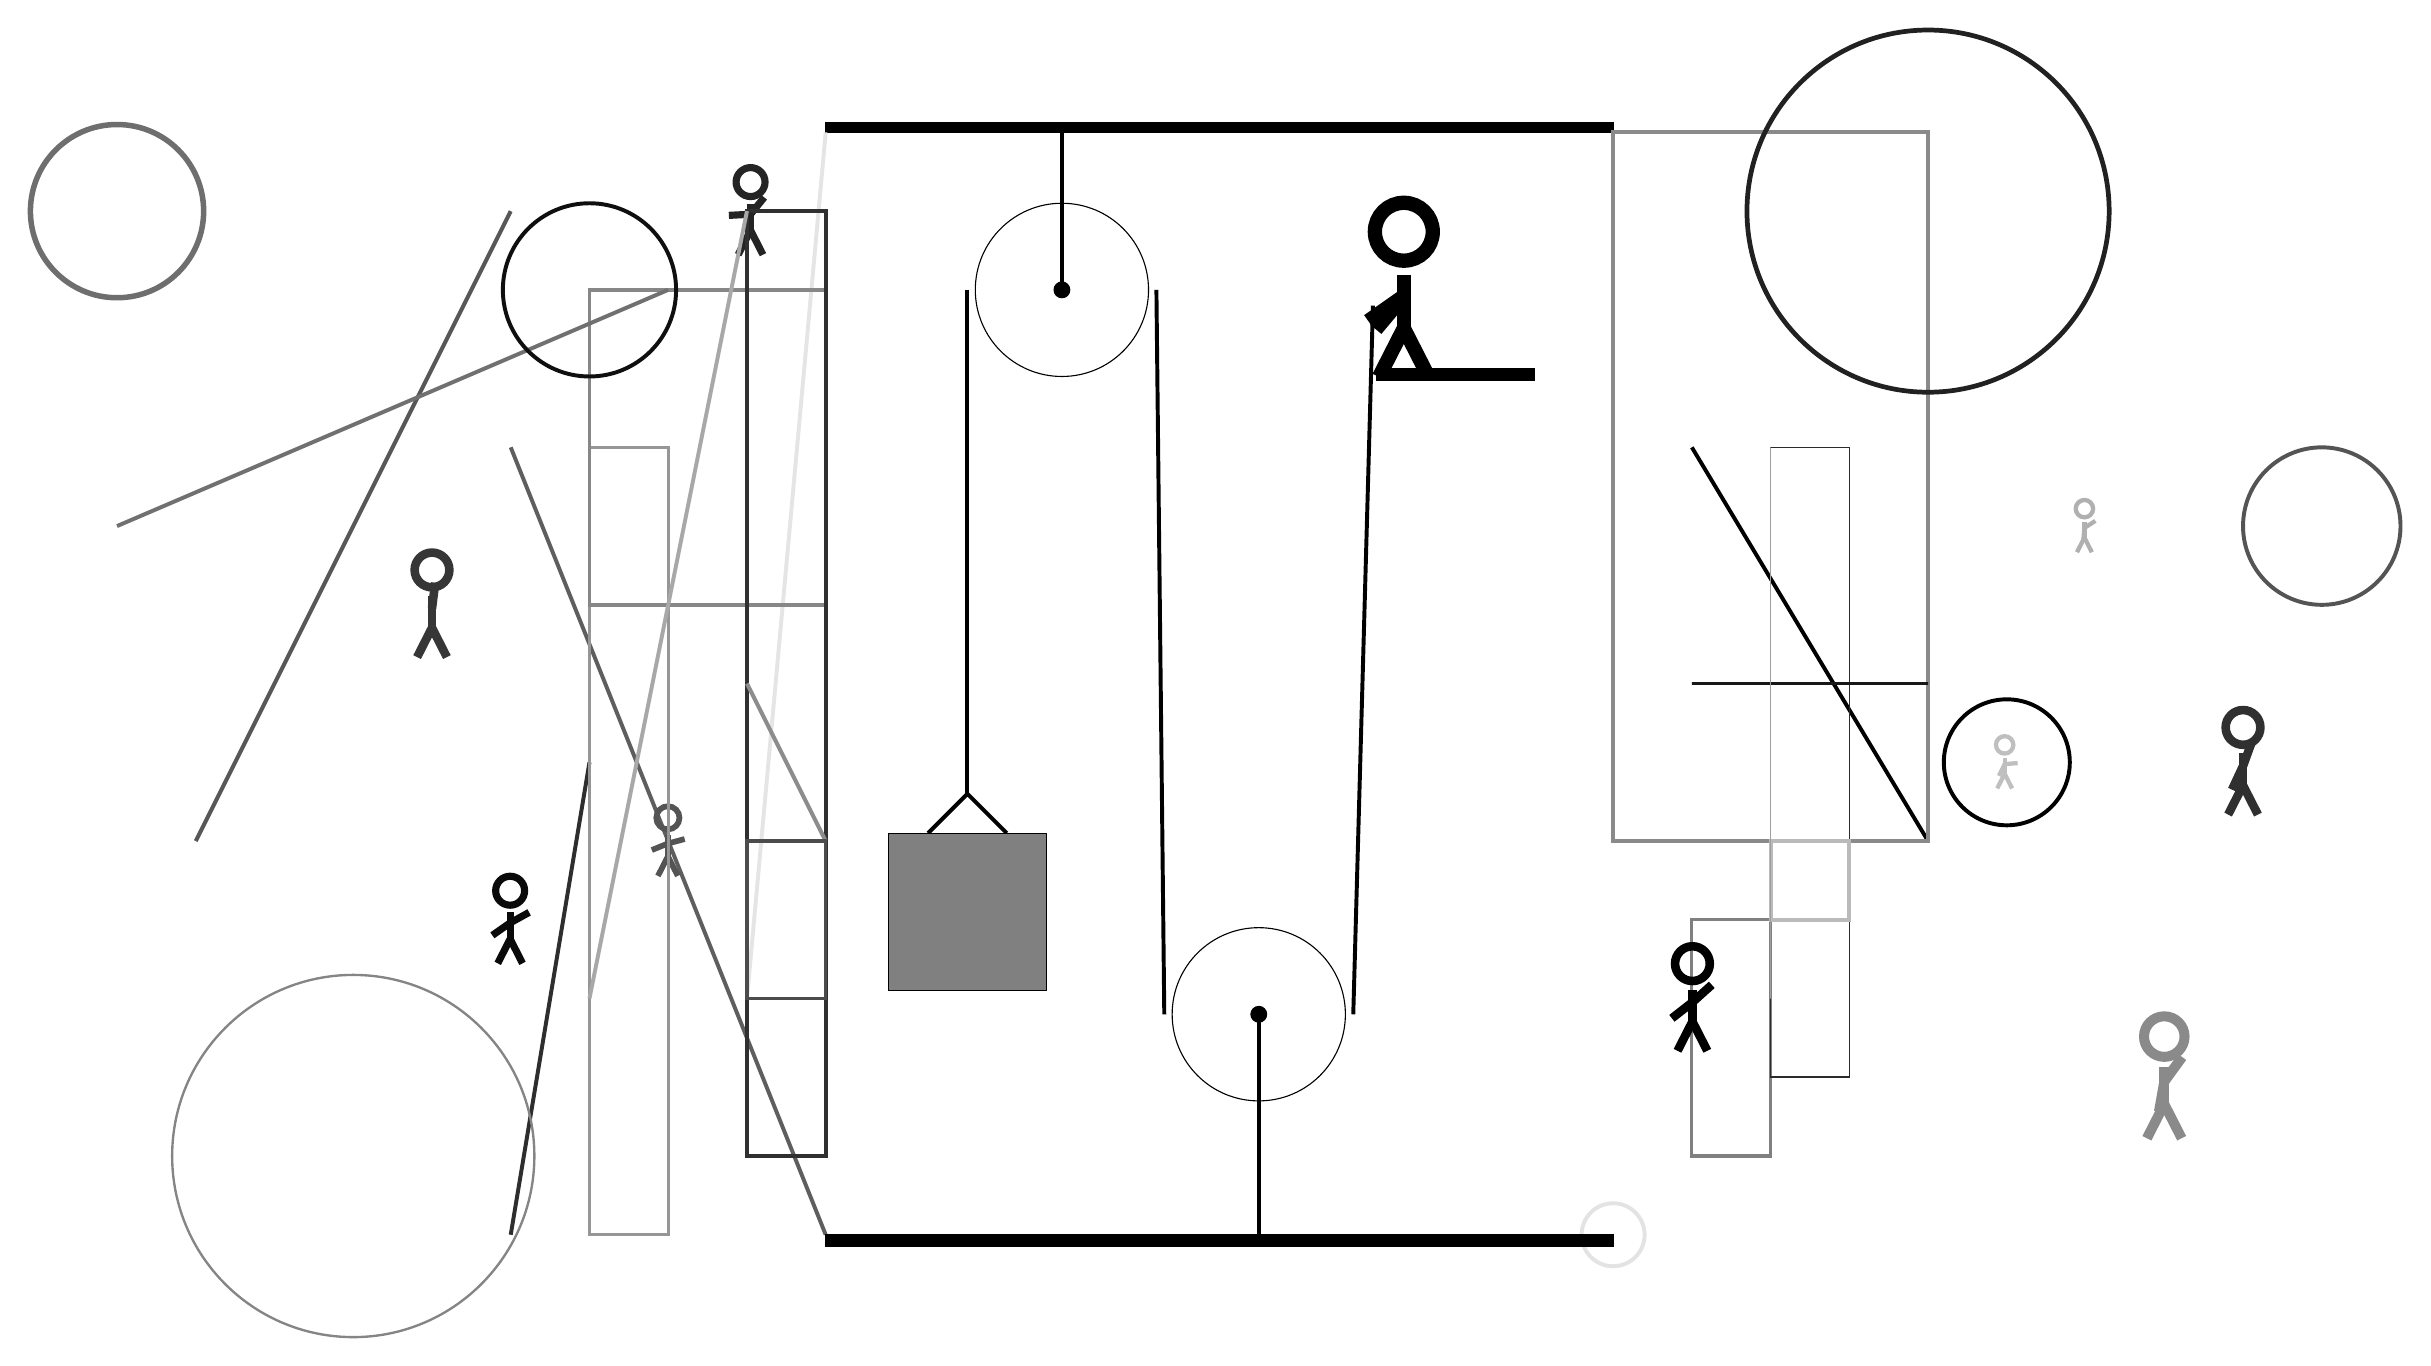
\begin{tikzpicture}
			%%%%% START %%%%%
			
			\draw[fill=black] (-2, 14) rectangle (8, 14.125);
			
			\draw (3.5, 2.8) circle (1.1);
			\draw[fill=black] (3.5, 2.8) circle (0.1);
			\draw[line width=0.5mm] (3.5, 2.8) -- (3.5, 0);
			
			\draw (1, 12) circle (1.1);
			\draw[fill=black] (1, 12) circle (0.1);
			\draw[line width=0.5mm] (1, 14) -- (1, 12);
			
			\draw[line width=0.5mm](-0.7, 5.1) --  (-0.2, 5.6) -- (0.3, 5.1);
			\draw[fill=black!50] (-1.2, 5.1) rectangle (0.8, 3.1);
			
			\draw[line width=0.5mm](-0.2, 12) -- (-0.2, 5.6);
			\centerarc[line width=0.5mm](1, 12)(180:0:1.2000000000000002)
			\draw[line width=0.5mm](2.2, 12) -- (2.3, 2.8);
			\centerarc[line width=0.5mm](3.5, 2.8)(180:360:1.2000000000000002)
			\draw[line width=0.5mm](4.7, 2.8) -- (4.95, 11.8);
			
			\node at (5.3, 12) {\Strichmaxerl[10][35][-130]};
			\draw[fill=black] (5, 11) rectangle (7, 10.85);
			
			\draw[line width=0.5mm, color=black!100](12, 5) -- (9, 10);
			
			\draw[line width=0.5mm, color=black!63](-2, 0) -- (-6, 10);
			\draw[line width=0.5mm, color=black!66](-6, 13) -- (-10, 5);
			\draw [line width=0.5mm, color=black!11](8, 0) circle (0.4);
			
			\draw [line width=0.5mm, color=black!100](13, 6) circle (0.8);
			
			\draw [line width=0.6mm, color=black!63](-8, 4) circle (0.0);
			\node[line width=0.5mm, color=black!67] at (-4, 5) {\Strichmaxerl[4][22][15]};
			
			\draw[line width=0.5mm, color=black!82](-5, 6) -- (-6, 0);
			\draw[line width=0.5mm, color=black!10](-3, 3) -- (-2, 14);
			
			\draw[line width=0.5mm, color=black!46] (8, 5) rectangle (12, 14);
			\node[line width=0.2mm, color=black!96] at (-6, 4) {\Strichmaxerl[5][35][29]};
			\node[line width=0.4mm, color=black!86] at (-3, 13) {\Strichmaxerl[5][3][51]};
			\draw[line width=0.4mm, color=black!41] (-4, 10) rectangle (-5, 0);
			
			\draw[line width=0.5mm, color=black!47] (-2, 12) rectangle (-5, 8);
			\draw[line width=0.5mm, color=black!81] (-3, 13) rectangle (-2, 1);
			\draw[line width=0.5mm, color=black!56](-4, 12) -- (-11, 9);
			\draw[line width=0.5mm, color=black!45](-3, 7) -- (-2, 5);
			\node[line width=0.7mm, color=black!46] at (15, 2) {\Strichmaxerl[7][80][54]};
			\draw [line width=0.3mm, color=black!48](-8, 1) circle (2.3);
			\node[line width=0.7mm, color=black!25] at (13, 6) {\Strichmaxerl[3][64][5]};
			\draw [line width=0.7mm, color=black!57](-11, 13) circle (1.1);
			
			\draw[line width=0.4mm, color=black!50] (10, 4) rectangle (9, 1);
			
			\draw [line width=0.6mm, color=black!87](12, 13) circle (2.3);
			\node[line width=0.7mm, color=black!100] at (9, 3) {\Strichmaxerl[6][38][42]};
			\draw[line width=0.2mm, color=black!83] (10, 10) rectangle (11, 2);
			\node[line width=0.4mm, color=black!79] at (-7, 8) {\Strichmaxerl[6][90][83]};
			\draw[line width=0.4mm, color=black!70] (-2, 3) rectangle (-3, 5);
			\draw[line width=0.5mm, color=black!27] (10, 5) rectangle (11, 4);
			\node[line width=0.5mm, color=black!81] at (16, 6) {\Strichmaxerl[6][65][70]};
			
			\draw [line width=0.5mm, color=black!67](17, 9) circle (1.0);
			\draw[line width=0.5mm, color=black!34](-3, 13) -- (-5, 3);
			\draw [line width=0.5mm, color=black!94](-5, 12) circle (1.1);
			\draw[line width=0.3mm, color=black!91] (9, 7) rectangle (12, 7);
			
			\draw[line width=0.2mm, color=black!38] (10, 3) rectangle (10, 10);
			\node[line width=0.5mm, color=black!31] at (14, 9) {\Strichmaxerl[3][85][33]};
			
			\draw[fill=black] (-2, 0) rectangle (8, -0.15);
			
			%%%%% END %%%%%
		\end{tikzpicture}
	\end{figure}	
\end{document}